\chapter{Literature Review - Speech Classification}\label{ch-lit-rev}
Having reviewed the acquisition and processing of speech-like signals, this text now seeks to define emotion from a speech signal context. While a number of features can be used to indicate an emotion present in a speech signal, (refer to table \ref{Emo_Char_Tab}), the CyTex transform is primarily (and almost solely) interested in pitch. However, it must be noted that classification is conducted on the basis of a deep learning framework. This means that manual feature extraction is not necessary. Although, the CyTex is a means of implicitly extracting certain features from an audio file. Different models of emotion are defined for reference within this chapter. This section also introduces the reader to SER from a high level, detailing each step of the process. Contemporary methods and models tested on well known SER datasets are briefly detailed. These modern studies function as comparative points to grade the success of CyTex relative to established approaches. Their implementation and results are primarily discussed. Finally, a number of the challenges facing current researchers are presented, some of which CyTex addresses.


% SECTION:
% ================================================
\section{Defining Emotion in Speech Signals}
Interestingly, no consensus definition of emotion exists in the psychological research community \cite{surveyCORE1}. Part of the reason may be the many ways to classify a concept as broad as emotion. By constraining the definition of emotion to one within the domain of speech, this definition becomes easier to construct, although less rigorous. However, the rigour used is sufficient for machine learning applications. Two models of emotion are considered, with varying simplicity and robustness. These models are the \textbf{discrete emotional model} and the \textbf{dimensional emotional model}.
\subsection{The Discrete Emotional Model}
Six prominent categories of emotions have been formulated as the "building blocks" of other emotions. These emotions consist of sadness, happiness, fear, anger, disgust and surprise, as suggested by \cite{ekman2013emotion}. In defining these as \textit{basic emotions}, it is implied that more complicated emotions are expressed as combinations of the basic emotions. While this model is simple and easy to interpret, some researchers believe it lacks the ability to clearly express more complicated emotions. This emotional model (or one tangential to it) is often used in the construction of emotional speech datasets like the EMODB dataset \cite{EMODB_97}. It allows for simple labelling of data and identification of the target classification. 

\subsection{The Dimensional Emotional Model}
This model of emotional state was developed to describe all emotional states \cite{RUSSELL1977}. This model opts for com[posing emotion of broad factors/dimensions. In particular, these include valence, arousal, control and power. In defining all emotions in terms of these dimensions, as opposed to separate base emotions, we can better define what makes an emotion. \cite{nicolaou2011} notes that most emotions can be characterised by two dimensions: valence and arousal. \textit{Valence} describes the positivity of an emotion, described in terms of pleasant or unpleasant. \textit{Arousal} details the relative strength of a particular emotion to the subject exhibiting that emotion. For example, anger would have a large arousal strength, where as an emotion like boredom would typically have a much smaller arousal strength. The use of arousal and valence as the defining criteria for emotional states is a popular two-dimensional model. Dominance/power may be included as a third dimensional to give a more robust model of emotion and further differentiate between emotions. This characteristic is effectively the perceived strength of a subject displaying an emotional reaction. Depending on the number of dimensions used, however, some emotions may appear as identical. One may obviously note that a large number of dimensions may be required to sufficiently describe all emotions. This is infeasible in a machine learning setting and as such there is an inherent trade off between dimensions and precision. Also, unlike the discrete emotional model, classification of emotions loses its ease of identification. 

\subsection{Prosodic Features of Emotional Speech}
Many SER systems utilise prosodic features for the classification of emotion in acoustic signals. These features are intuitive for humans as they form the basis for verbal communication. All verbal speakers are familiar with features like pitch, intensity and speaking rate. A sufficient summary of prosodic features is detailed in table \ref{Emo_Char_Tab} and related to corresponding emotions that exhibit such features, (excerpted from \cite{Ramakrishnan12}). Contemporary literature has previously demonstrated a preference for the use of prosodic features, as they yield more distinct properties than their non-prosodic counterparts. In particular, \cite{zeng2009} notes that a large amount of research in this field points to pitch (fundamental frequency) and energy forming the largest basis for recognising emotion.
\begin{table}[h]
% [h] argument will place the table here approximately.
% centering not working so use negative hspace instead!
    % \centering
    \hspace*{-2.5cm}
    \begin{tabular}{|l||p{2cm}|p{2cm}|p{2cm}|p{2cm}|p{2cm}|}\hline
        \backslashbox[14em]{\textbf{Characteristics}}{\textbf{Emotions}}
        & \textbf{JOY} & \textbf{ANGER} & \textbf{SADNESS} & \textbf{FEAR} & \textbf{DISGUST}\\\hline\hline
        Pitch Mean &High &Very High &Very Low &Very High &Very Low\\\hline
        Pitch Range &High &High &Low &High &High-male, Low-female\\\hline
        Pitch Variance &High &Very High &Low &Very High &Low\\\hline
        Pitch Contour &Incline &Decline &Decline &Incline &Decline\\\hline
        Intensity Mean &High &Very High-male, High-female& Low& Med/High &Low\\\hline
        Intensity Range &High &High &Low &High &Low\\\hline
        Speaking Rate & High & Low-male, High-female & High-male, Low-female & High & Very low-male, Low-female\\\hline
        Transmission Durability &Low &Low &High &Low &High\\\hline
        Voice Quality &Modal/tense &Breathy; med blaring timbre &Resonant timbre &Falsetto &Resonant timbre\\\hline
    \end{tabular}
    \caption{Emotional Acoustic Characteristics \cite{Ramakrishnan12}}
    \label{Emo_Char_Tab}
\end{table}


% SECTION:
% ================================================
\section{Speech Emotion Recognition - An Overview}
SER encompasses the methods and techniques employed to detect emotion(s) within speech signals. The core inclusion of an SER system is some supervised learning model which seeks to classify these emotions. Figure \ref{ser_branch_fig} illustrates a broad view of some of the major considerations of building an SER system. Generally, in working through an SER related task, one would traverse from left to right in this diagram. While not every sub-branch is necessary for successful implementation, each should be considered.
\begin{figure}[h]
        \hspace{-1cm}
        % \centering
        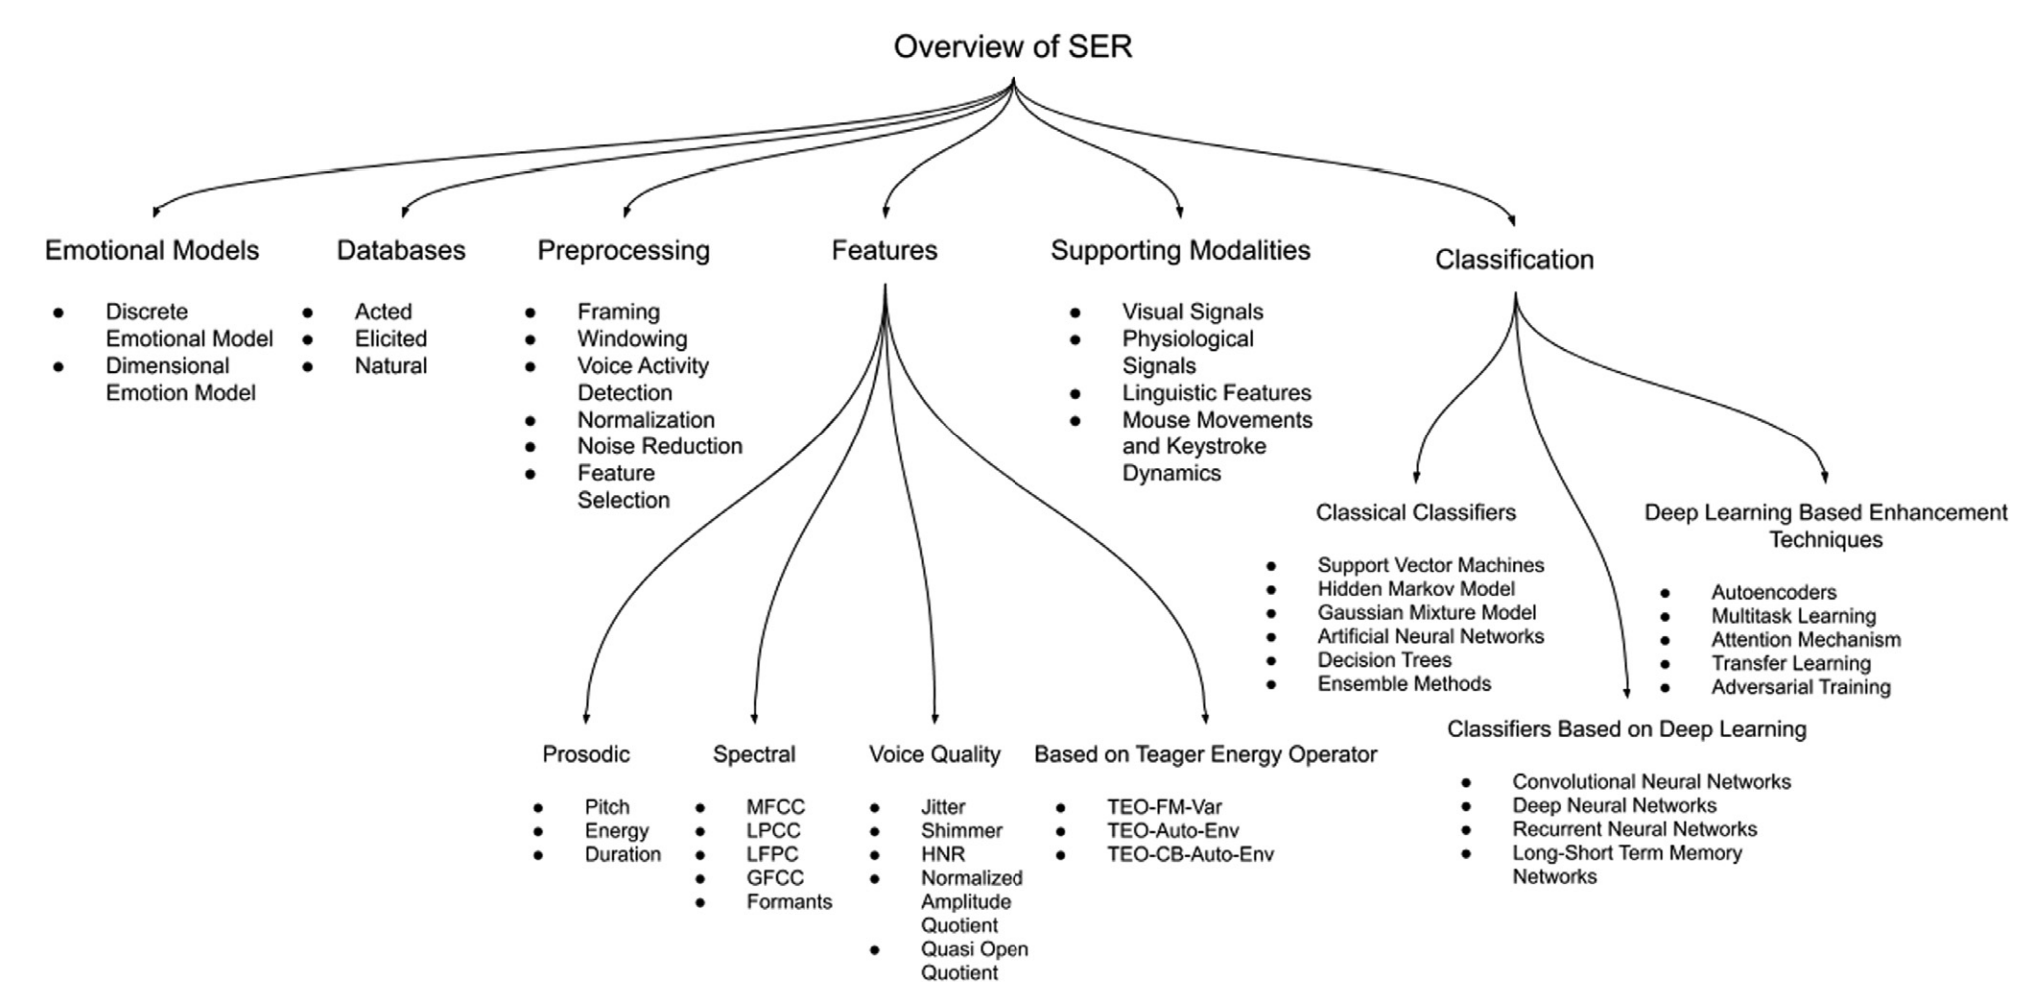
\includegraphics[scale = 1.0]{images/SER Overview Map.png}
        \caption{SER Overview \cite{surveyCORE1}}
        \label{ser_branch_fig}
\end{figure}
 Different models for emotion have been discussed in detail in the sections prior and the databases of SER are detailed in chapter \ref{ch-theory}. The CyTex transform itself serves as a means of employing preprocessing and preliminary feature extraction, also discussed in chapter \ref{ch-theory}. Supporting modalities are other media which support a classifier in determining which emotion is present in a data sample. This may involve things like video and facial motion capture. However, this study is solely interested in the analysis of acoustic audio data. As such, supporting modalities will not be addressed within this thesis. A number of classification schemes can be utilised in SER, including traditional machine learning approaches or advanced deep learning approaches. This study employs a deep learning approach based on a convolutional neural network architecture and utilises transfer learning for model enhancement. Both of these topics are discussed in further detail in chapter \ref{ch-theory}.\\ \\
 Figure \ref{ser_pipeline_fig} details a similar, albeit simplified, framework for the implementation of an SER system. Here the signal source will be some acoustic signal from a labelled emotional audio dataset. Feature extraction synthesises key identifiers of emotional from the signal source. Post processing is used to 'clean' the format of the incoming signal prior to selecting which features to use for training and classification. Following this, a machine learning model is trained and employed as a means of classifying data. It should be noted that a more common approach is to implement some form of preprocessing initially and then perform feature extraction and selection in a single step. When using a deep learning model as a classifier, feature extraction and selection can be discounted entirely.
\begin{figure}[h]
        \centering
        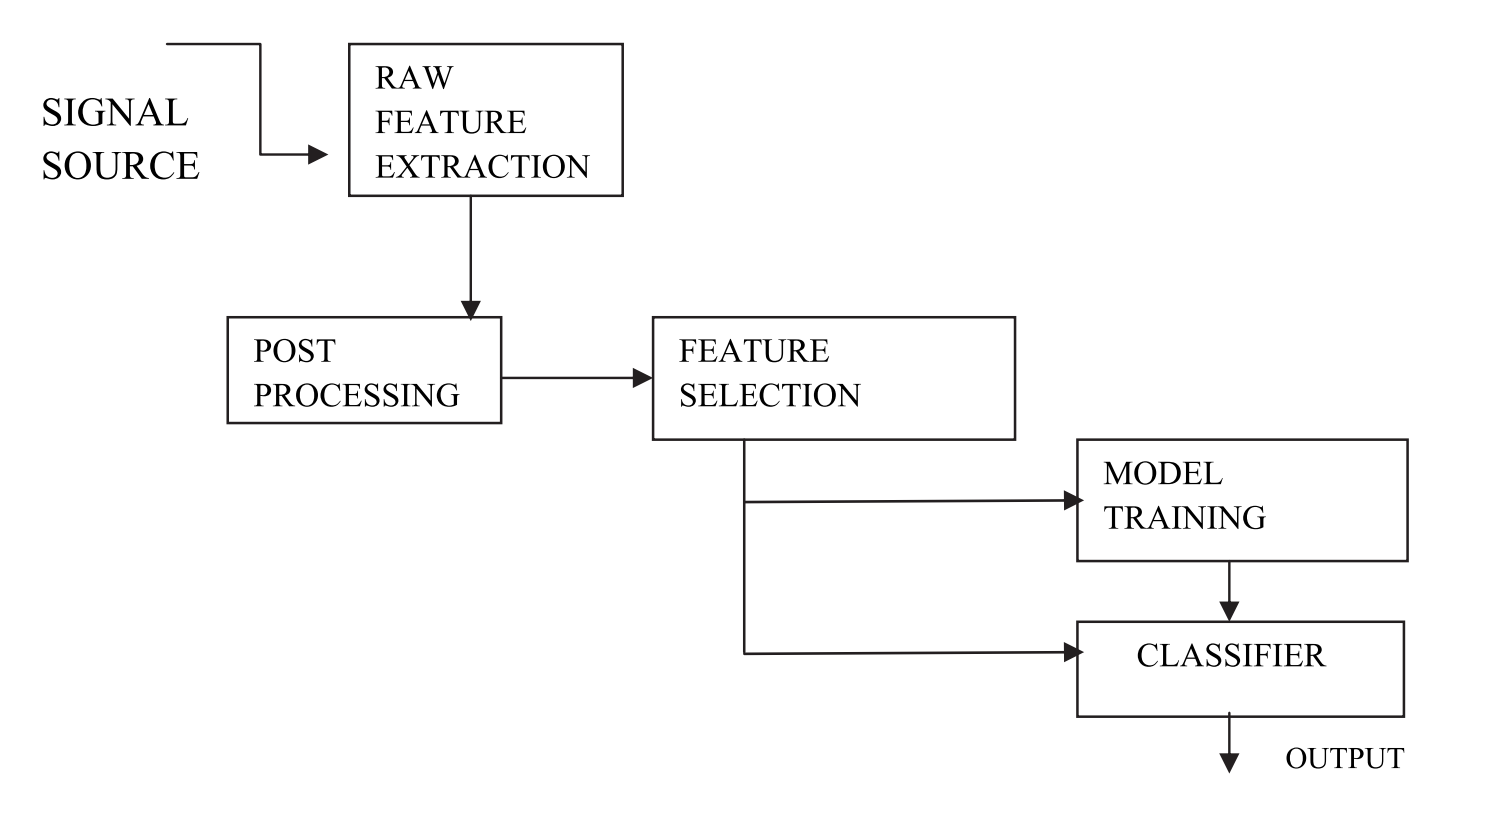
\includegraphics[scale = 1.0]{images/Basic SER framework.png}
        \caption{Basic SER Framework \cite{Ramakrishnan12}}
        \label{ser_pipeline_fig}
\end{figure}

\subsection{SER Using Deep Learning}
In this study a deep learning algorithm is used to classify the emotion of acoustic signals. This deep learning algorithm is trained on CyTex images, defined in chapter \ref{ch-theory}. While the CyTex images perform some kind of feature extraction, these features are not explicitly provided to the deep learning model. With advancements in technology and its access, the popularity of deep learning has increased. This increase in the application of deep learning usage has also seen improvements in results on benchmark SER datasets. As noted previously, deep learning possesses the benefit of requiring no manual extraction or selection of features from the data. The deep learning model will automatically 'learn' which features provide the best means of classification.


% SECTION:
% ================================================
\section{Benchmarks \& Contemporary Methods}
The two key datasets that this dissertation aims to focus on are the EMODB and RAVDESS datasets. To give a fair point of comparison for the developed model's performance other benchmark methods have been studied for the same datasets. Methods highlighted employ novel schemes and have achieved high accuracy on their respective datasets. Not all methods utilised in contemporary studies will be rigorously define. Readers are encouraged to to access the provided reference papers of contemporary methods for more comprehensive explanations on applied procedures. This section merely highlights general strategies and the prominent results of each case.

\subsection{Stacked Autoencoder Network \& Deep Belief Network}
Two models are constructed by Zhou et al. harnessing a Stacked Autoencoder (SAE) network and a Deep Belief Network (DBN) \cite{zhou2016deep}. In using deep learning, emotional feature extraction is automated, reducing complexity of implementation and eliminating subjectivity of feature selection. Audio files from the EMODB dataset are used as direct inputs into the model. Preprocessing begins with signal sampling at $16kHz$. This is followed by dividing the data into $50ms$ frames (to be considered stationary) via Hamming windowing. Each Hamming window has a length of 256 and contains an overlap percentage of $50\%$. Following this the frames are divided into a training and test set and fed into the deep learning model. This process is depicted in figure \ref{zhou2016_flowchart}.\\ \\
\begin{figure}[h]
        \centering
        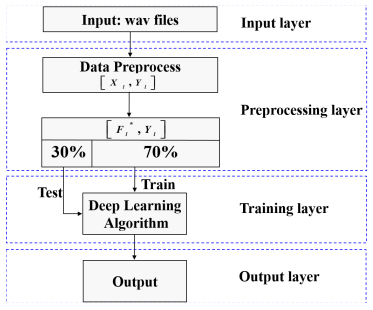
\includegraphics[scale = 0.8]{images/zhou_flowchart_fig.png}
        \caption{SER via Direct Signal Learning \cite{zhou2016deep}}
        \label{zhou2016_flowchart}
\end{figure}
In the SAE approach, autoencoders are placed in a sequential pipeline. Following this, parameters are fine tuned and autoencoders are stacked in a network. The DBN is based on a Restricted Boltzmann Machine (RBM). RBM's are trained and also pipelined. After stacking these machines and retraining several times, one obtains a DBN.\\ \\
During testing on the EMODB dataset, recognition accuracy reached a height of $65.00\%$ for both models (although the stacked autoencoder approach was marginally lower). However, in this case the number of predicted emotional states was reduced to two. Both models demonstrated significantly worse performance when required to predict seven emotional states. The SAE model exhibited an accuracy of $25\%$, while the DBN demonstrated an accuracy of $38\%$. While this accuracy is significantly lower than the other methods discussed in this paper, it is still important. This result contextualises the performance of deep learning when applied directly to audio signals. Such results also suggest that both methods of feature extraction do not yield salient enough features for the basis of classification.

\subsection{Deep 1D \& 2D CNN-LSTM Networks}
Zhao et al. employs two different CNNs and LSTMs and compares the two systems. The first of the two CNNs (1D) aims to model local emotional features extracted from the speech signal itself. The second CNN (2D) analyses log-mel spectrogram images to learn features that more globally describe the emotional content of a signal \cite{ZHAO2019}. Models share closely related architectures containing four local feature learning blocks (LFLBs). Each of these blocks are composed of a convolutional layer, batch normalization layer, exponential linear unit layer and finally a max-pooling layer. These blocks are proceeded by a single LSTM layer in each case. The LSTM layers specialise in learning long-term dependencies, which in the case of log-mel spectrogram approaches, is traditionally lacking. This counteracts the frequency/time trade-off of log-mel spectrogram generation to some degree. Figure \ref{zhao2019_arch_fig} illustrates a block diagram comprised of the discussed blocks.\\ \\
\begin{figure}[h]
        \centering
        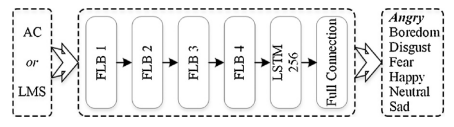
\includegraphics[scale = 1.0]{images/zhao_architecture.png}
        \caption{1D and 2D CNN-LSTM Architectures \cite{ZHAO2019}}
        \label{zhao2019_arch_fig}
\end{figure}
The training and validation results of the two-dimensional CNN-LSTM architecture are displayed in figure \ref{zhao2019_train_fig}. The largest validation accuracy achieved for the EMODB dataset was $76.64\%$. After validating and testing the data on the EMODB dataset, an average accuracy of $95.33\%$ was achieved through use of the two-dimensional model. The one-dimensional model performed less favourably, achieving an average accuracy of $86.73\%$. These metrics were found by retrieving the confusion matrix of classification rates across all emotion types and averaging the correct prediction percentages for each. This result is one of the highest benchmarks on this dataset in recent years. Exemplary results were also demonstrated on the IEMOCAP database. An accuracy of $89.16\%$ was achieved utilising the same two-dimensional CNN-LSTM approach. 
\begin{figure}[h]
        \centering
        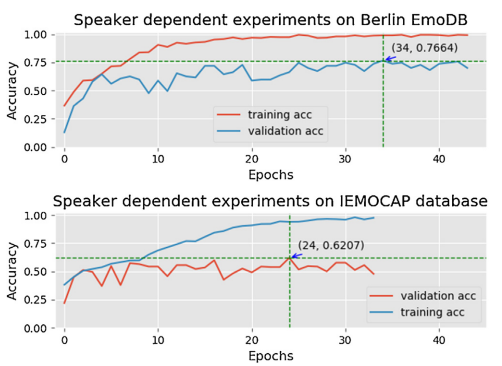
\includegraphics[scale = 0.8]{images/Zhao-2dCNN_trainvalResults.png}
        \caption{2D CNN LSTM train-val Accuracy \cite{ZHAO2019}}
        \label{zhao2019_train_fig}
\end{figure}

\subsection{3D CNN for Spectro-Temporal Feature Learning}
The addition of LSTM blocks to the output of CNN systems introduces increased model complexity. In attempts to capture important temporal data, without the addition of LSTM blocks, Kim et al. presents an additional dimension in a CNN architecture \cite{kim2017speech}. These three-dimensional CNN structures are capable of simultaneous short and long-term spectral feature extraction. Such models were found to be more effective than other methods in the domain of spectro-temporal feature extraction and classification. Figure \ref{3dcnn_fig} depicts a two-dimensional CNN which is fed into LSTM layers (a), and a three-dimensional CNN. In (a), a 2D convolution is applied to each spectral image (feature map). These spectral feature maps are arranged in time (annotated L). By applying a 3D convolution to a time series of feature maps, we preserve the three-dimensional structure of the input. \\ \\
\begin{figure}[h]
        \centering
        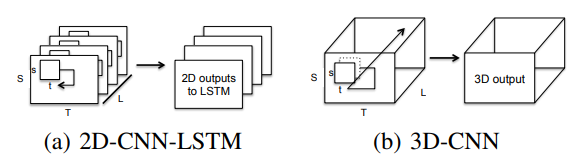
\includegraphics[scale = 0.8]{images/3dcnn_IMG.png}
        \caption{Differing Dimensions of CNN Architectures \cite{kim2017speech}}
        \label{3dcnn_fig}
\end{figure}
The dataset used for the training and validation of this approach was created by aggregating seven other SER datasets. Thus, the specific accuracy metrics are not provided for the EMODB, RAVDESS or IEMOCAP datasets. This approach did, however, outperform a number of \textit{'off the shelf'} methods on the constructed dataset, like those proposed in \cite{ZHAO2019}.


% Check definition of speaker independent???
% \subsection{A Speaker Independent SVM Approach}
% \cite{Shirani2016}

\subsection{Novel Temporal Emotional Modeling - TIM\_NET}
Temporal-aware bI-direction Multi-scale Network (TIM-Net) details a network capable of temporal learning on different time scales. Information from both the past and future instances of a signal are used to enhance feature representation \cite{ye2023temporal}. This appraoch seeks to remedy some common drawbacks of LSTM implementation. Specifically, an inability to capture long-term dependencies which inform context. Mel-Frequency Cepstral Coefficients (MFCCs) were chosen as inputs for the model. Framing and windowing is applied to inputs, utilising a Hamming window. The first 39 coefficients are utilised after further processing. The key method exploited in this system is the use of temporal-aware blocks which, in parallel, process forwards and backwards time cases of the input. These blocks analyse a number of consecutive frames and select the most affective. A causal constraint is applied to ensure the elimination of leakage from future to past samples. Feature outputs from the forward and backward direction paths are fused dynamically using weighted summation. The net process is represented in figure \ref{timnet_fig}, also further detailing the temporal-aware blocks.\\ \\
\begin{figure}[ht]
        % \hspace{-2.5cm}
        \centering
        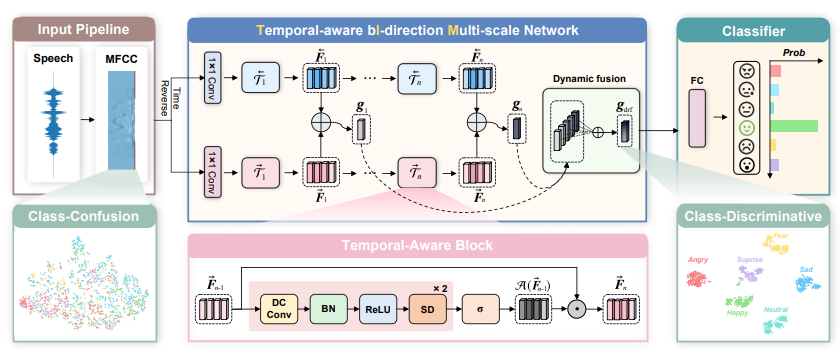
\includegraphics[scale = 0.8]{images/TIM_NET_fig.png}
        \caption{TIM-Net Framework for SER \cite{ye2023temporal}}
        \label{timnet_fig}
\end{figure}
TIM-Net has demonstrated exceptional results over a number of standard datasets within the SER community. Of interest for comparison to this study and those previously mentioned, the EMODB, RAVDESS and IEMOCAP databases are all utilised. Accuracy is measured using both Unweighted Average Recall (UAR) and Weighted Average Recall (WAR). The WAR measures seek to compensate for the imbalance of classes in some datasets. However, only the UAR results are noted here as they are directly comparable to the average accuracy specified in other contemporary methods. For the EMODB dataset, a UAR score of $95.17\%$ was achieved, existing in the same neighbourhood as other state of the art solutions. TIM-Net is one of the highest performing models on the RAVDESS dataset, demonstrating an average accuracy of $91.93\%$. Finally, this model achieved a $72.5\%$ UAR score on the IEMOCAP database. 


% \subsection{CNN-Assisted Enhanced Audio Signal Processing}
% \cite{kwon2020_cnn-assist}

% SECTION:
% ================================================
\section{Speech Processing Challenges}
Speech emotion recognition is still juvenile in the context of machine learning fields. This entails periods of rapid advancement, but comes with the disadvantages of numerous obstacles that the field is yet to overcome. Some of these are discussed subsequently and are recommended as further areas of research into the future of the SER field.

\subsection{Databases}
Any machine learning system is only as good as the data it is trained on. However, it is very difficult to approximate life-like emotional speech datasets for reasons discussed in chapter \ref{ch-theory}. Many of these reasons involve the legality of capturing real emotional responses. Those datasets that attempt to create more realistic emotional responses are often incomplete (emotionally) and are difficult to label. Annotation, in these circumstances, may introduce error into the dataset as the recognition rate is at or below $90\%$ \cite{surveyCORE1}.\\ \\
The validation of a model's performance is also dependant on its underlying database. Comparison between the performance of different models can prove difficult as models may be specialised for particular databases, or trained on separate ones altogether. \cite{zeng2009} notes the requirement of research communities unionising to formulate common evaluation procedures on comparative datasets. This will better allow for comparison of models and indicate their relative proficiency. 

\subsection{Cultural Barriers}
A universal SER model seems like an impossibility. A number of studies, attempt to recognise emotion for different languages. However, these methods typically exhibit lower accuracy than speaker dependent methods. The obvious caveat to methods that use prosodic features, for instance, is tonal languages. In non-tonal languages, features like pitch provide formative grounds for the classification of emotions. Whereas a tonal language utilises pitch to imply the meaning of speech, rather than the emotional state.

\subsection{Multi-Speech Recognition}
Further work should be conducted in the domain of identifying which signal, in a composition, a machine should focus on. In a real-world setting, it is likely that environments will be noisy and contain numerous acoustic signals. Algorithms that separate speech from ambient noise or other speech singals can be implemented in preprocessing, however, \textit{"current systems fail to notice this problem"} \cite{surveyCORE1}.
 
\subsection{Pre-trained Model Limitations}
Finally, that which CyTex and other image processing based approaches addresses, is the lack of pre-trained models able to be utilised for speech emotion recognition. This introduces a barrier into the field of SER as many methodologies require the construction and training of entirely new models. By converting audio signals to an image domain, a wealth of pre-trained and openly accessible deep learning models may be used.
